\documentclass[11pt]{article}

\usepackage{amsmath,amssymb,amsthm,mathtools}
\usepackage[margin=1in]{geometry}
\usepackage{booktabs}
\usepackage{graphicx}
\usepackage[colorlinks=true,linkcolor=blue,citecolor=blue]{hyperref}

\newtheorem{theorem}{Theorem}[section]
\newtheorem{proposition}[theorem]{Proposition}
\newtheorem{lemma}[theorem]{Lemma}
\newtheorem{corollary}[theorem]{Corollary}
\newtheorem{definition}[theorem]{Definition}
\newtheorem{assumption}[theorem]{Assumption}
\theoremstyle{remark}
\newtheorem{remark}[theorem]{Remark}

\newcommand{\R}{\mathbb{R}}
\newcommand{\E}{\mathbb{E}}
\newcommand{\relu}{\sigma}
\newcommand{\norm}[1]{\left\lVert #1 \right\rVert}
\newcommand{\abs}[1]{\left\lvert #1 \right\rvert}
\newcommand{\ip}[2]{\left\langle #1, #2 \right\rangle}
\DeclareMathOperator{\diag}{diag}
\DeclareMathOperator{\Tr}{Tr}

\title{Merge-Based Structured Pruning:\\ a Geometric Theory with Certified and
Expected-Error Guarantees}
\author{Working notes (theory companion to \texttt{studies/DESIGN\_SPACE.md})}
\date{August 2026}

\begin{document}
\maketitle

\begin{abstract}
We develop, from first principles, a theory of structured pruning by
\emph{merging} units of a ReLU layer. The theory proceeds in five steps:
(1) a canonical, gauge-invariant parameterization of a ReLU unit as an
oriented hyperplane with a loudness weight; (2) an associative merge operator
on units that is exact on coincident units and whose pointwise error is
localized to activation-disagreement regions; (3) a certified worst-case error
bound whose accumulation is a valid stopping budget and whose squared form is
the Ward clustering objective; (4) an average-case theory in the Hilbert space
$L^2(\mu)$ of unit functions, in which merge damage, optimal fan-out repair,
and the whole selection problem have closed forms under Gaussian input
measures; (5) the identification of subset-plus-least-squares pruning
(OBS/OSSCAR) as the medoid special case of the framework, which yields an
adaptive method spanning both regimes. Every theorem is stated with its
assumptions; a final section confronts each claim with the empirical record
(E1--E13) and reports where assumptions failed and what that implied.
\end{abstract}

\tableofcontents

%======================================================================
\section{Setting and notation}\label{sec:setting}

We consider one prunable layer of a feed-forward network. The layer receives
inputs $x \in \R^d$, contains $H$ ReLU units, and feeds a linear consumer.

\begin{definition}[Layer, units, consumer]\label{def:layer}
Unit $i \in \{1,\dots,H\}$ has incoming weights $w_i \in \R^d$, bias
$b_i \in \R$, and activation
\[
  h_i(x) \;=\; \relu(w_i^\top x + b_i), \qquad \relu(t) = \max\{0,t\}.
\]
The consumer reads the layer through columns $c_i \in \R^m$ (row $i$ of the
next weight matrix, transposed), producing the pre-activation contribution
\[
  F(x) \;=\; \sum_{i=1}^{H} c_i\, h_i(x) \;\in\; \R^m .
\]
\end{definition}

\begin{remark}[Convolutions]\label{rem:conv}
For a Conv$\to$BN$\to$ReLU block in evaluation mode, fold the BatchNorm into
effective weights $w^{\mathrm{eff}} = (\gamma_{\mathrm{bn}}/
\sqrt{\sigma^2_{\mathrm{run}}+\epsilon})\,w$ and
$b^{\mathrm{eff}} = \beta_{\mathrm{bn}} - \gamma_{\mathrm{bn}}
\mu_{\mathrm{run}}/\sqrt{\sigma^2_{\mathrm{run}}+\epsilon}$ (exact), let $x$
range over im2col \emph{patches}, and let $c_i$ be the flattened kernel slice
of the consumer conv (or the head column after global average pooling, which
is linear per channel). Weight sharing means each \emph{filter} is a single
unit on patch space; every statement below applies verbatim.
\end{remark}

Throughout, $x_0 \in \R^d$ is a reference point and $R_0 > 0$ a radius such
that all admissible inputs satisfy $\norm{x - x_0} \le R_0$ (for images: the
center and enclosing radius of the per-feature input box; for deeper layers:
propagated bounds or calibration ranges). Only the \emph{domain} $(x_0,R_0)$
is assumed known in the worst-case theory; the average-case theory of
Section~\ref{sec:functional} additionally uses an input \emph{measure} $\mu$.

%======================================================================
\section{Canonical parameterization and gauge}\label{sec:param}

\begin{definition}[Canonical coordinates]\label{def:coords}
For a unit with $\norm{w} > 0$ define
\[
  \alpha = \norm{w} \quad (\text{gain}), \qquad
  u = w/\norm{w} \quad (\text{orientation}), \qquad
  \rho = -b/\norm{w} \quad (\text{signed offset}),
\]
\[
  \gamma = u^\top x_0 - \rho \quad (\text{signed margin at } x_0), \qquad
  a = \alpha \norm{c} \quad (\text{loudness}).
\]
The unit's pre-activation in normalized form is
$s(x) = u^\top x - \rho = u^\top (x - x_0) + \gamma$, so that
$h(x) = \alpha\,\relu(s(x))$ and the activation boundary is the hyperplane
$\{x : s(x)=0\}$, at signed distance $\gamma$ from $x_0$ along $u$.
\end{definition}

\begin{lemma}[Gauge invariance and completeness]\label{lem:gauge}
For every $t>0$ the reparameterization $(w,b,c) \mapsto (tw, tb, c/t)$ leaves
the contribution $c\,h(x)$ unchanged for all $x$. The invariants of this gauge
action are exactly $(u, \rho, \alpha c)$; equivalently $(u,\gamma,\alpha c)$.
\end{lemma}

\begin{proof}
By positive homogeneity, $\relu(t z) = t\,\relu(z)$ for $t > 0$, so
$(c/t)\relu(tw^\top x + tb) = c\,\relu(w^\top x + b)$. Under the action,
$u$ and $\rho$ are fixed and $\alpha c \mapsto (t\alpha)(c/t) = \alpha c$.
Conversely $(u,\rho,\alpha c)$ determines $c\,h(x) =
(\alpha c)\,\relu(u^\top x - \rho)$, hence determines the orbit.
\end{proof}

\begin{lemma}[Sign-blindness of anchors]\label{lem:anchor}
The anchor $\beta \coloneqq -(b/\norm{w})\, w/\norm{w} = \rho\, u$ (the foot of
the perpendicular from the origin to the boundary) is invariant under
$(w,b)\mapsto(-w,-b)$, although this flip replaces the unit by its
complementary unit (active on the opposite half-space). Moreover all
boundaries through the origin have $\beta = 0$ regardless of orientation.
Hence $\beta$ alone does not determine the unit; the pair $(u,\gamma)$ does.
\end{lemma}

\begin{proof}
Under the flip, $\rho \mapsto -\rho$ and $u \mapsto -u$, so
$\beta = \rho u$ is fixed, while the active half-space
$\{s > 0\}$ is replaced by its complement. If $\rho = 0$ then $\beta = 0$ for
every $u$.
\end{proof}

\begin{remark}[The covector cylinder]\label{rem:cylinder}
Encode a unit by $\tilde q = (R_0 u, \gamma) \in \R^{d+1}$. Since
$\norm{R_0 u} = R_0$, all units live on the cylinder
$S^{d-1}(R_0)\times\R$: angular position is the boundary's orientation
(sign included --- complementary units are antipodal), height is the
boundary's placement relative to the data. $\tilde q$ is the coefficient
vector of the affine map $\delta \mapsto s(x_0 + R_0\delta)$ on the unit
ball, so Euclidean proximity of $\tilde q$'s controls uniform proximity of
pre-activations (Theorem~\ref{thm:bound} makes this exact). This is the
classical parameterization of oriented hyperplanes (in $d=2$, Hough space).
\end{remark}

%======================================================================
\section{The merge operator}\label{sec:merge}

Fix per-unit weights $a_i > 0$ (we will use the loudness $a_i =
\alpha_i\norm{c_i}$; the theory below holds for any positive weights).

\begin{definition}[Cluster merge]\label{def:merge}
For a cluster $C \subseteq \{1,\dots,H\}$ define the \emph{covector sums}
\[
  S_u = \sum_{i\in C} a_i u_i, \qquad
  S_\rho = \sum_{i\in C} a_i \rho_i, \qquad
  S_c = \sum_{i\in C} \alpha_i c_i .
\]
If $S_u \ne 0$, the \emph{merged unit} is
\[
  \bar u = S_u/\norm{S_u}, \qquad
  \bar\rho = S_\rho/\norm{S_u}, \qquad
  \text{realized as } \bar h(x) = \relu(\bar u^\top x - \bar\rho)
\]
with consumer column $\bar c = S_c$ (\emph{sum rule}; refined in
Section~\ref{sec:repair}). The merged contribution is
$\bar F_C(x) = S_c\,\relu(\bar s(x))$, $\bar s(x) = \bar u^\top x - \bar\rho$.
\end{definition}

\begin{proposition}[Associativity]\label{prop:assoc}
Encode each unit by $\xi_i = a_i(u_i,\rho_i) \in \R^{d+1}$ and each merged
unit by $\bar\xi = \norm{S_u}(\bar u,\bar\rho)$. Then $\bar\xi =
\sum_{i\in C}\xi_i$, and likewise $S_c$ is additive. Consequently merging is
associative and order-independent: any sequence of pairwise merges whose
final partition is $\mathcal{P}$ produces exactly the units obtained by
merging each block of $\mathcal{P}$ at once.
\end{proposition}

\begin{proof}
$\norm{S_u}\,\bar u = S_u$ and $\norm{S_u}\,\bar\rho = S_\rho$ by
Definition~\ref{def:merge}, so $\bar\xi = (S_u, S_\rho) = \sum \xi_i$.
Vector addition is associative and commutative; the realized parameters are a
function of the sums only.
\end{proof}

\begin{proposition}[First-moment conservation]\label{prop:moment}
The total covector $\Xi = \sum_{k} \xi_k$ (sum over current units, merged or
not) and the total column sum $\sum_k \bar c_k$ are invariant under any
sequence of merges. So is the ``orientation energy''
$\sum_k A_k R_0^2 \norm{\bar u_k}^2 = R_0^2 \sum_i a_i$
(where $A_k$ is the block's weight sum), since every realized orientation is
unit-norm.
\end{proposition}

\begin{proof}
Immediate from Proposition~\ref{prop:assoc} and additivity of the weights.
\end{proof}

\begin{theorem}[Exactness on coincident units, arbitrary fan-out]
\label{thm:exact}
If all units of $C$ share one boundary and side, $(u_i,\rho_i) = (u,\rho)$
for all $i\in C$, then $\bar F_C(x) = F_C(x)$ for \emph{every} $x\in\R^d$ and
\emph{arbitrary} columns $c_i$ (any signs, any directions).
\end{theorem}

\begin{proof}
$S_u = (\sum a_i)\,u$, hence $\bar u = u$, $\bar\rho =
(\sum a_i\rho)/\sum a_i = \rho$. All units and the merged unit share the
indicator $\mathbf{1}\{u^\top x > \rho\}$; on the active set,
$F_C(x) = \sum_i c_i\alpha_i (u^\top x - \rho) = S_c\,(u^\top x-\rho)
= \bar F_C(x)$, and both vanish elsewhere.
\end{proof}

\begin{theorem}[Pointwise error identity; scalar, slope-matched case]
\label{thm:identity}
Let $m = 1$, $a_i \ge 0$, $f_C(x) = \sum_{i\in C} a_i \relu(s_i(x))$, and let
the merged unit be slope-matched: $\bar f_C(x) = \relu\!\big(\sum_i a_i
s_i(x)\big)$. Then for all $x$,
\[
  f_C(x) - \bar f_C(x)
  \;=\; \sum_{i\in C} a_i \relu(s_i(x)) - \relu\!\Big(\sum_{i\in C} a_i
  s_i(x)\Big) \;\ge\; 0,
\]
with equality whenever all $s_i(x)$ share a sign. Consequently the error is
supported on the \emph{activation-disagreement region}
$D_C = \{x : \exists\, i,j \in C,\ s_i(x) > 0 > s_j(x)\}$, a union of wedges
between the cluster's boundaries.
\end{theorem}

\begin{proof}
Nonnegativity is subadditivity of $\relu$ on nonnegative combinations:
$\relu(\sum a_i s_i) \le \sum a_i \relu(s_i)$ by convexity and positive
homogeneity. If all $s_i(x) \ge 0$ both sides equal $\sum a_i s_i(x)$; if
all $s_i(x)\le 0$ both sides vanish.
\end{proof}

\begin{corollary}[Saturation as the degenerate case]\label{cor:saturation}
If $\gamma_i \le -R_0$ then $s_i(x) = u_i^\top(x-x_0) + \gamma_i \le 0$ on the
whole domain: the unit is identically zero there and its removal is exact.
If $\gamma_i \ge R_0$ the unit is \emph{affine} on the domain,
$h_i(x) = \alpha_i(u_i^\top x - \rho_i)$, and can be absorbed exactly by any
consumer able to represent affine functions of $x$ (in practice: folded into
downstream weights and biases). Dead-unit deletion, always-on folding, and
redundancy merging are thus one mechanism: all are instances of
Theorem~\ref{thm:identity} with empty or trivial disagreement region.
\end{corollary}

\begin{remark}[Sum rule vs.\ slope matching]\label{rem:overshoot}
The realized sum rule of Definition~\ref{def:merge} gives, in the scalar
case, $\bar f = A_C\,\relu(\tilde u^\top x - \tilde\rho)$ with
$\tilde u = S_u/A_C$, which \emph{overshoots} the slope-matched unit by the
factor $A_C/\norm{S_u} \ge 1$ (equality iff all $u_i$ coincide); the factor
is $1 + O(\varepsilon_u^2)$ for angular dispersion $\varepsilon_u$. The
projection update of Section~\ref{sec:repair} removes the overshoot
optimally; the identity above is exact for the slope-matched realization.
\end{remark}

%======================================================================
\section{Certified worst-case error}\label{sec:certified}

\begin{theorem}[Certified merge bound, fan-out, centered]\label{thm:bound}
Let $C$ be merged as in Definition~\ref{def:merge} with column
$\bar c = S_c$. Then for every $x$ with $\norm{x - x_0}\le R_0$,
\[
  \norm{F_C(x) - \bar F_C(x)}
  \;\le\; \sum_{i\in C} \alpha_i \norm{c_i}\,
  \Big( R_0 \norm{u_i - \bar u} + \abs{\gamma_i - \bar\gamma} \Big),
  \qquad \bar\gamma \coloneqq \bar u^\top x_0 - \bar\rho .
\]
\end{theorem}

\begin{proof}
Since $\bar c = \sum_i \alpha_i c_i$,
\[
  F_C(x) - \bar F_C(x)
  = \sum_i \alpha_i c_i\big[\relu(s_i(x)) - \relu(\bar s(x))\big].
\]
ReLU is $1$-Lipschitz, so $\abs{\relu(s_i)-\relu(\bar s)} \le
\abs{s_i - \bar s}$. Writing $x = x_0 + \delta$, $\norm{\delta}\le R_0$,
\[
  s_i(x) - \bar s(x) = (u_i-\bar u)^\top \delta + (\gamma_i - \bar\gamma),
\]
and Cauchy--Schwarz gives $\abs{s_i - \bar s} \le R_0\norm{u_i - \bar u} +
\abs{\gamma_i - \bar\gamma}$. The triangle inequality over $i$ completes the
proof.
\end{proof}

\begin{remark}
The bound holds for \emph{every} admissible input --- it is a certificate,
not an expectation --- and it is computable from weights plus the domain
$(x_0,R_0)$ alone. Its accumulated value over all merged clusters is the
stopping budget used by the pipeline. Centering at $x_0$ (rather than the
origin) is essential in deep layers, where inputs are far from the origin.
\end{remark}

\begin{proposition}[Ward form of the bound]\label{prop:ward}
For a pair $\{i,j\}$ merged at the weighted mean of the covectors
$\tilde q_k = (R_0 u_k, \gamma_k)$ with weights $a_k$, the bound of
Theorem~\ref{thm:bound} evaluates to
$\tfrac{2 a_i a_j}{a_i + a_j}\,d_1(i,j)$ with
$d_1(i,j) = R_0\norm{u_i - u_j}\cdot\lambda + \abs{\gamma_i-\gamma_j}\cdot
(1-\lambda)$-type mean splits; more useful is the squared version: merging
weighted points $\{(a_k, \tilde q_k)\}$ at their weighted mean reduces the
weighted second moment $\sum_k a_k \norm{\tilde q_k}^2$ by exactly the
\emph{Ward cost}
\[
  \frac{a_i a_j}{a_i + a_j}\, \norm{\tilde q_i - \tilde q_j}^2
\]
(parallel-axis theorem). Greedy smallest-Ward-cost merging is therefore
greedy minimization of a squared relative of the certified bound, and the
accumulated second-moment loss of the covector cloud equals the accumulated
Ward cost, independent of merge order.
\end{proposition}

\begin{proof}
Parallel axis: for weights $m_k$ and points $p_k$ with weighted mean
$\bar p$ and $M=\sum m_k$,
$\sum m_k\norm{p_k}^2 - M\norm{\bar p}^2 = \sum m_k \norm{p_k - \bar p}^2$;
for two points the right side is
$\tfrac{m_1 m_2}{M}\norm{p_1 - p_2}^2$ by direct expansion. Order
independence follows from associativity of the weighted mean with additive
weights.
\end{proof}

\begin{remark}[What the realized merge does to spectra]\label{rem:spectra}
The realized merged covector is the sphere projection of the centroid
($\bar u$ is unit-norm), so: the first covector moment is conserved
\emph{exactly} (Proposition~\ref{prop:moment}); the orientation block of the
weighted second moment is conserved \emph{mechanically}; and the
parallel-axis identity for the remaining part holds to second order in
cluster dispersion. Hence ``spectral stability of the layer'' is meaningful
only for the \emph{loudness-weighted, centered} second moment; unweighted or
anchor-based Grams change even under exact merges (they lose the multiplicity
$a_i$) and are dominated by large-$\abs\gamma$ (saturated, functionally
irrelevant) units.
\end{remark}

\begin{proposition}[Composition across layers]\label{prop:compose}
Let the network be $f = g_\ell \circ f_\ell$ where $f_\ell$ contains the
pruned layer and $g_\ell$ (the downstream network) is $L_\ell$-Lipschitz on a
set containing the reachable sets of both the original and pruned $f_\ell$.
If each pruned layer $\ell$ incurs error at most $\varepsilon_\ell$ in the
consumer's pre-activation (uniformly on its admissible inputs), then
\[
  \norm{\hat f(x) - f(x)} \;\le\; \sum_{\ell} L_\ell\, \varepsilon_\ell
  \qquad \text{for all admissible } x,
\]
where $\hat f$ prunes all layers and $L_\ell$ is the Lipschitz constant of
everything downstream of layer $\ell$'s consumer.
\end{proposition}

\begin{proof}
Telescope: replace one layer at a time,
$\hat f - f = \sum_\ell \big(f^{(\le \ell)} - f^{(\le \ell-1)}\big)$ where
$f^{(\le \ell)}$ prunes layers $1..\ell$. Each summand differs only in layer
$\ell$; its norm is at most $L_\ell \varepsilon_\ell$ by the Lipschitz
property, provided $\varepsilon_\ell$ holds on the (possibly shifted) inputs
reaching layer $\ell$ --- guaranteed when the domain radius used for
$\varepsilon_\ell$ covers the pruned network's reachable set, e.g.\ by
enlarging $R_0$ by the accumulated upstream error.
\end{proof}

%======================================================================
\section{Average-case theory: the functional Hilbert space}
\label{sec:functional}

Worst-case bounds defend every point of the domain equally; an
\emph{average-case} theory weights inputs by a probability measure $\mu$ on
$\R^d$ with finite second moments.

\begin{definition}[Unit functions and kernel]\label{def:kernel}
Let $h_i(x) = \alpha_i \relu(u_i^\top x - \rho_i) \in L^2(\mu)$ and define
the kernel
$K_{ij} = \ip{h_i}{h_j}_{L^2(\mu)} = \E_\mu[h_i(x) h_j(x)]$.
For layer contributions, the relevant Gram is
$\widetilde K_{ij} = (c_i^\top c_j)\,K_{ij}$, since
$\E\norm{\sum_i c_i h_i}^2 = \sum_{ij} \widetilde K_{ij}$.
\end{definition}

\begin{proposition}[Exact expected merge damage]\label{prop:damage}
Replacing $\{(c_i,h_i)\}_{i\in C}$ by a single unit $(\bar c, \bar h)$ incurs
\[
  \E_\mu\Big\lVert \sum_{i\in C} c_i h_i - \bar c\, \bar h \Big\rVert^2
  = \sum_{i,j\in C} (c_i^\top c_j) K_{ij}
  - 2\sum_{i\in C} (c_i^\top \bar c)\, \ip{h_i}{\bar h}
  + \norm{\bar c}^2 \ip{\bar h}{\bar h},
\]
a closed quadratic form in kernel evaluations. In particular the exact
expected damage of every candidate pair merge --- and of any surgery ---
is computable without forward passes once $K$ is available.
\end{proposition}

\begin{proof} Expand the square and exchange expectation with the finite
sums. \end{proof}

\subsection{Closed forms under Gaussian measures}

Let $\mu = \mathcal N(\mu_0, \Sigma)$. Each pre-activation
$t_i = u_i^\top x - \rho_i$ is Gaussian with mean
$m_i = u_i^\top \mu_0 - \rho_i$ and covariance
$\mathrm{Cov}(t_i,t_j) = u_i^\top \Sigma u_j$; hence every kernel entry
reduces to the bivariate quantity
$G(a,b,c) = \E[(X-a)_+(Y-b)_+]$ for standard bivariate normal $(X,Y)$ with
correlation $c$, via
$K_{ij} = \alpha_i\alpha_j\, s_i s_j\, G(-m_i/s_i,\, -m_j/s_j,\,
\mathrm{corr}(t_i,t_j))$, $s_i^2 = u_i^\top\Sigma u_i$.

\begin{theorem}[Closed form of $G$]\label{thm:G}
Let $s = \sqrt{1-c^2} > 0$, $\varphi,\Phi$ the standard normal density and
cdf, $\bar\Phi = 1-\Phi$, $\beta_a = (b-ca)/s$, $\alpha_b = (a-cb)/s$, and
$L(a,b;c) = \Pr(X>a, Y>b)$. Then
\[
  G(a,b,c) = (c + ab)\, L(a,b;c)
  \;-\; b\,\varphi(a)\bar\Phi(\beta_a)
  \;-\; a\,\varphi(b)\bar\Phi(\alpha_b)
  \;+\; s\,\varphi(b)\varphi(\alpha_b).
\]
Special cases: $G(a,a,1) = (1+a^2)\bar\Phi(a) - a\varphi(a)$;
$G(0,0,\cos\theta) = \tfrac{1}{2\pi}\big(\sin\theta +
(\pi-\theta)\cos\theta\big)$, the arc-cosine kernel of Cho--Saul.
\end{theorem}

\begin{proof}
Write $Y = cX + sZ$ with $Z \perp X$ standard normal, and let
$\mathbf 1 = \mathbf 1\{X>a, Y>b\}$. Expanding
$G = \E[XY\mathbf 1] - b\,\E[X\mathbf 1] - a\,\E[Y\mathbf 1] + ab\,L$, it
suffices to compute the truncated moments. The key identity
\[
  \varphi(x)\,\varphi\!\big(\tfrac{b - cx}{s}\big)
  = \varphi(b)\,\varphi\!\big(\tfrac{x - cb}{s}\big)
\]
follows by completing the square in the exponent. Using it:
(i) $\E[X\mathbf 1] = \varphi(a)\bar\Phi(\beta_a) +
c\,\varphi(b)\bar\Phi(\alpha_b)$, by integration by parts on
$\int_a^\infty x\varphi(x)\bar\Phi(\tfrac{b-cx}{s})dx$;
(ii) $\E[Y\mathbf 1] = \varphi(b)\bar\Phi(\alpha_b) +
c\,\varphi(a)\bar\Phi(\beta_a)$ by symmetry;
(iii) $\E[XZ\mathbf 1] = s\,\varphi(b)\big(cb\,\bar\Phi(\alpha_b) +
s\,\varphi(\alpha_b)\big)$, obtained by conditioning on $X$
($\E[Z\,\mathbf 1\{Z > g(X)\} \mid X] = \varphi(g(X))$ with
$g(x) = (b-cx)/s$), substituting the key identity, and evaluating
$\int_a^\infty x\,\varphi\big(\tfrac{x-cb}{s}\big)dx =
s\big(cb\,\bar\Phi(\alpha_b) + s\,\varphi(\alpha_b)\big)$;
(iv) $\E[X^2\mathbf 1] = L + a\varphi(a)\bar\Phi(\beta_a) +
c\,\varphi(b)\big(cb\,\bar\Phi(\alpha_b) + s\varphi(\alpha_b)\big)$, by parts
using $\tfrac{d}{dx}(-\varphi) = x\varphi$. Then
$\E[XY\mathbf 1] = c\,\E[X^2\mathbf 1] + s\,\E[XZ\mathbf 1]
= cL + ca\varphi(a)\bar\Phi(\beta_a) + cb\varphi(b)\bar\Phi(\alpha_b) +
s\varphi(b)\varphi(\alpha_b)$, using $c^2 + s^2 = 1$. Assembling the four
moments yields the stated formula. For $c=1$, $Y=X$ and
$G(a,a,1)=\E[(X-a)_+^2]$ evaluates directly; for $a=b=0$,
$L(0,0;c) = \tfrac14 + \tfrac{\arcsin c}{2\pi}$ gives the arc-cosine form.
\end{proof}

\begin{remark}[Which Gaussian?]\label{rem:measure}
Three instantiations, in decreasing ignorance:
(i) \emph{isotropic}: $\Sigma = \tfrac{R_0^2}{d+2} I$, matching the second
moments of the uniform ball (for $z$ uniform on $B_{R_0}$,
$\E[(u^\top(z-x_0))^2] = R_0^2/(d+2)$);
(ii) \emph{product/box}: $\Sigma = \diag(r^2/3)$ from per-feature ranges;
(iii) \emph{matched}: $(\mu_0,\Sigma)$ estimated from unlabeled calibration
inputs. The choice is the entire empirical risk of the average-case theory:
the formulas are exact \emph{under} $\mu$, and mis-specified $\mu$ produces
confidently wrong scores (Section~\ref{sec:evidence}, E2/E4/E10). Trained
units aim at correlated input directions, so any product measure
underestimates the variance of $t_i$; full covariance is the minimum
sufficient correction, and for strongly non-Gaussian inputs (conv patches:
a point mass of background plus sparse rectified foreground) even matched
Gaussians fail and the empirical measure must be used.
\end{remark}

%======================================================================
\section{Optimal fan-out repair}\label{sec:repair}

Merging fixes the surviving \emph{units}; the consumer's columns remain free.
All repairs below are orthogonal projections in $L^2(\mu)$ and therefore
optimal in expected squared error under $\mu$.

\begin{proposition}[Per-cluster projection]\label{prop:proj}
Given the merged unit $\bar h$, the column minimizing
$\E\norm{\sum_{i\in C} c_i h_i - \bar c\,\bar h}^2$ is
\[
  \bar c^\star = \frac{\sum_{i\in C} c_i \ip{h_i}{\bar h}}
  {\ip{\bar h}{\bar h}} .
\]
For $m=1$ and the choice $a_i = \alpha_i c_i > 0$ this reduces to the
slope-matched rule of Theorem~\ref{thm:identity} up to $O(\varepsilon^2)$
(and exactly in the co-active region).
\end{proposition}

\begin{proof}
The objective is a quadratic in $\bar c$ minimized coordinate-wise by
projecting each output coordinate onto $\mathrm{span}\{\bar h\}$.
\end{proof}

\begin{theorem}[Global least-squares repair]\label{thm:global}
Let $\{\hat h_k\}_{k=1}^{K}$ be the surviving (merged or original) units and
$G^{kk}_{k\ell} = \ip{\hat h_k}{\hat h_\ell}$,
$G^{ko}_{k i} = \ip{\hat h_k}{h_i}$. The columns minimizing
$\E\norm{\sum_i c_i h_i - \sum_k \hat c_k \hat h_k}^2$ solve the normal
equations
\[
  G^{kk}\, \widehat C \;=\; G^{ko}\, C ,
\]
with $\widehat C, C$ the matrices of columns. Under Gaussian $\mu$ every
entry of $G^{kk}, G^{ko}$ is a closed-form evaluation of
Theorem~\ref{thm:G}; under the empirical measure of $N$ samples the same
equations are ridge least squares on activations (the repair used by
OBS-family methods).
\end{theorem}

\begin{proof}
Orthogonal projection of the vector-valued function $\sum_i c_i h_i$ onto
$\mathrm{span}\{\hat h_1,\dots,\hat h_K\}$, coordinate-wise in the output
index.
\end{proof}

\begin{corollary}[Bias compensation]\label{cor:bias}
If the consumer has a bias (or the next normalization layer can absorb a
constant), replacing it by $b + \E_\mu[\text{residual}]$ further reduces the
expected squared error by $\norm{\E_\mu[\text{residual}]}^2$, by the
mean/centered orthogonal decomposition. For the slope-matched merge, the
residual is pointwise nonnegative (Theorem~\ref{thm:identity}), so this
correction is systematically nonzero. Under Gaussian $\mu$,
$\E[\relu(t)] = s\,\varphi(m/s) + m\,\Phi(m/s)$ gives it in closed form.
\end{corollary}

\begin{remark}[Parametric vs.\ empirical Grams]\label{rem:estimators}
The two instantiations of Theorem~\ref{thm:global} differ only in the
estimator of the Gram matrices: analytic under a fitted $\mu$
($O(d^2)$ parameters, well-conditioned, exactly correct iff $\mu$ is), versus
empirical from $N$ samples (unbiased for the true measure, rank $\le N$,
variance-limited). When second moments are sufficient statistics of the true
input distribution the two coincide as $N$ grows and the parametric form
regularizes at small $N$; when the input law is far from Gaussian the
parametric form is inconsistent and the empirical form must be preferred.
This single dichotomy explains the architecture split in the empirical
record (E9 vs.\ E10).
\end{remark}

%======================================================================
\section{Relation to OBS-family pruning (OSSCAR)}\label{sec:osscar}

Subset-selection methods choose a support $S \subseteq \{1..H\}$, zero the
complement, and re-solve the consumer on $S$: with empirical Gram
$H = X^\top X$ (consumer inputs $X$) and target $G = HB$, they minimize the
quadratic $Q(W) = \tfrac12 \Tr(W^\top H W) - \Tr(G^\top W)$ over $W$
supported on $S$'s rows.

\begin{proposition}[OBS removal score]\label{prop:obs}
Let $W^\star = H^{-1}G$ be the unconstrained minimizer and let unit $j$ own
one row (the group case is analogous with block inverses). The minimal
objective increase from constraining $W_j = 0$, with all other rows
re-optimized, is
\[
  \Delta Q_j \;=\; \tfrac12\, \frac{\norm{W^\star_j}^2}{[H^{-1}]_{jj}} .
\]
\end{proposition}

\begin{proof}
Minimize $Q(W^\star + \Delta)$ over $\Delta$ subject to
$e_j^\top(W^\star+\Delta) = 0$. Since $\nabla Q(W^\star)=0$, the increase is
$\tfrac12\Tr(\Delta^\top H \Delta)$; the Lagrangian stationarity gives
$\Delta = -H^{-1}e_j \lambda^\top$ with
$\lambda = W^{\star\top} e_j / [H^{-1}]_{jj}$, and substituting yields the
stated value.
\end{proof}

\begin{remark}[Placement inside the framework]\label{rem:placement}
(i) OSSCAR's repair \emph{is} Theorem~\ref{thm:global} under the empirical
measure. (ii) Its selection score is \emph{conditional} (cost of removal
given optimal compensation), whereas the merge costs of
Sections~\ref{sec:certified}--\ref{sec:functional} are local; its swap stage
partially restores global optimality. (iii) Its dictionary is the
\emph{subset} family: exactly the special case of
Definition~\ref{def:merge} in which each cluster is realized by a member
(medoid) rather than the mean. Consequently: where genuine clusters exist,
mean realization strictly enlarges the dictionary (and empirically wins,
E8); where they do not, mean units interpolate between dissimilar detectors
and the medoid/subset realization is correct (E10--E13). The adaptive rule
--- mean when the cluster's certificate (Theorem~\ref{thm:bound}) is small,
medoid otherwise --- contains both.
\end{remark}

%======================================================================
\section{The operating pipeline}\label{sec:pipeline}

\textbf{Selection.} Build the merge dendrogram greedily: repeatedly merge
the pair (cluster) of minimal cost, where cost is the Ward form
(Proposition~\ref{prop:ward}; domain knowledge only) or the exact expected
damage (Proposition~\ref{prop:damage} under the best available $\mu$). By
Proposition~\ref{prop:assoc} the trajectory is a dendrogram: every width is
a prefix, computed once.

\textbf{Realization.} Per cluster: mean unit (Definition~\ref{def:merge})
when its certified dispersion is small, medoid otherwise. Fan-out: global
repair (Theorem~\ref{thm:global}) with the Gram estimator matched to the
input law (parametric for MLP-type inputs; empirical for conv patches),
plus bias compensation (Corollary~\ref{cor:bias}); optionally one swap
refinement pass over the support (Section~\ref{sec:osscar}).

\textbf{Stopping.} Accumulate the certificate of Theorem~\ref{thm:bound}
(and/or the expected damage) and stop at a budget; per-layer budgets compose
by Proposition~\ref{prop:compose}. Thresholding pairwise similarity is
strictly dominated: it cannot control accumulation and its scale is
layer-dependent.

\textbf{Tiers.} The same pipeline degrades gracefully with information:
domain only $\to$ Ward costs + certificate (fully data-free);
$+\,O(d^2)$ moments from $\approx 10^2$ unlabeled inputs $\to$ closed-form
expected damage and repair; $+$ raw calibration activations $\to$ empirical
Grams and swap refinement (OBS-equivalent repair).

%======================================================================
\section{Confrontation with the empirical record}\label{sec:evidence}

Each theoretical claim above was tested; the ledger (E1--E13, in
\texttt{studies/DESIGN\_SPACE.md}) is summarized against the theory. Numbers
are medians over seeds; ``capacity'' is the fraction of units removable
within a stated accuracy budget.

\begin{center}
\small
\begin{tabular}{@{}p{0.33\textwidth}p{0.62\textwidth}@{}}
\toprule
Theory & Evidence \\
\midrule
Certificate (Thm~\ref{thm:bound}) tracks true damage &
E1: Spearman $0.99$--$1.0$ between accumulated bound and measured layer
error, all datasets. E6: as an \emph{absolute} threshold it transfers across
seeds/layers within a dataset (0.6--0.77 of oracle capacity at zero
violations) but its pessimism factor is domain-dependent --- ordering is
certified, calibration is per-domain. \\[2pt]
Conservation laws (Prop~\ref{prop:moment}) &
E1: first moment conserved to $2\times10^{-16}$; orientation-block energy
conserved mechanically (this \emph{predicted} the blindness of trace-based
spectral stopping rules, confirmed). \\[2pt]
Exactness and identity (Thms~\ref{thm:exact},~\ref{thm:identity}) &
E3: machine-precision on coincident units with arbitrary fan-out;
associativity verified bit-wise. \\[2pt]
Ward $=$ squared certificate (Prop~\ref{prop:ward}) &
E1/E7: greedy Ward selection is the robust domain-only policy; its costs are
\emph{not} comparable across layers (worst-case units), so cross-layer
allocation must use expected damage or equal fractions (E7). \\[2pt]
Measure choice is the whole risk (Rem~\ref{rem:measure}) &
E2: isotropic $\mu$ collapses on MNIST layer~0 (real projection spread
$2.3\times$ the model). E4: product measures also fail; matched covariance
repairs it and dominates (27--2--1 vs.\ Ward on layer error). E10: on conv
patches even matched Gaussians fail (kernel repair degrades $2$--$3\times$
faster than empirical at identical structure). \\[2pt]
Moment sufficiency (Rem~\ref{rem:estimators}) &
E9: on MLPs, parametric and empirical Grams give \emph{identical} capacities
at $N{=}128$ in every cell --- second moments capture everything the samples
know. E10: the same comparison fails on patches --- non-Gaussianity, as
predicted by the dichotomy. \\[2pt]
Global repair (Thm~\ref{thm:global}) &
E8: $+15$--$22$ points of joint capacity over the sum rule on MLPs at equal
data; exceeds the allocation \emph{oracle} under the old surgery ---
repair dominates allocation. \\[2pt]
Dictionary placement (Rem~\ref{rem:placement}) &
E8: mean realization beats medoid/survivor by $+7$--$12$ points where
clusters exist (MLPs). E11: removal sets of our selection and OSSCAR overlap
far above chance (up to $0.94$ vs.\ $0.50$). E12/E13: medoid $+$ empirical
LS $+$ swap on our supports reaches \emph{exact} OSSCAR parity on CNNs
(gap decomposition: surgery $+0.31$, greedy myopia $+0.07$, remainder $0$). \\[2pt]
Saturation corollary (Cor~\ref{cor:saturation}) &
Beta-saturation study: data-free certificates for dead/always-on units;
BatchNorm suppresses saturation (zero certified-saturated filters in conv
nets), so the merging channel carries conv pruning. \\[2pt]
Composition (Prop~\ref{prop:compose}) &
E7: joint pruning of all layers loses almost nothing relative to per-layer
capacities (64--70\% of all hidden units at $-1$pt on MLPs); intact-model
dendrograms suffice (sequential recomputation adds nothing). \\
\bottomrule
\end{tabular}
\end{center}

\subsection{Key results in figures and tables}

\begin{figure}[t]
\centering
\begin{minipage}{0.49\textwidth}\centering
  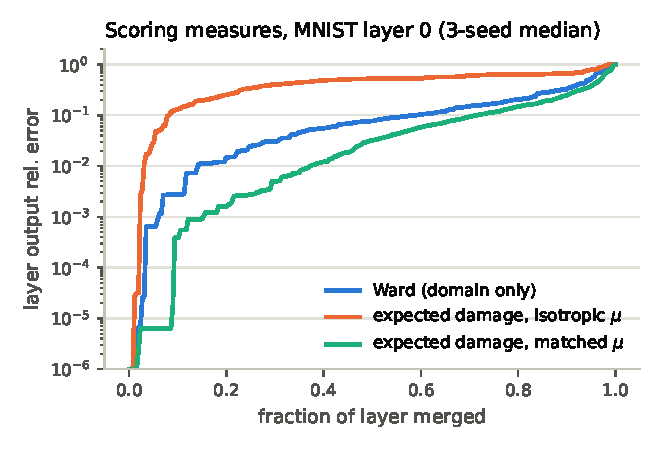
\includegraphics[width=\linewidth]{figs/fig_metric.pdf}
\end{minipage}\hfill
\begin{minipage}{0.49\textwidth}\centering
  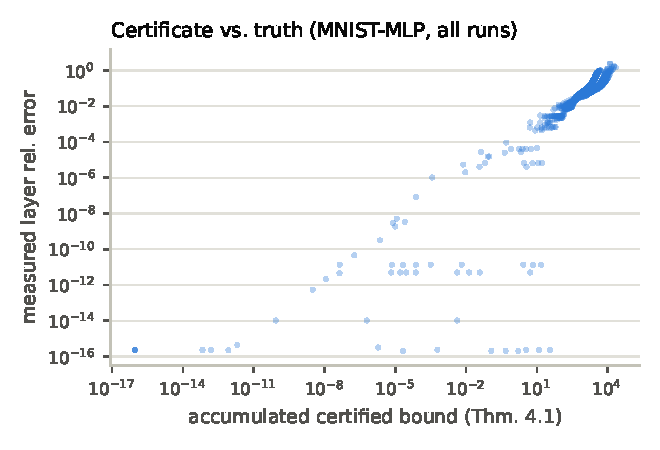
\includegraphics[width=\linewidth]{figs/fig_bound.pdf}
\end{minipage}
\caption{\textbf{Left (E2/E4):} the measure is the whole risk of the
average-case theory. On MNIST layer~0 the isotropic measure merges
``confidently wrong'' (error explodes almost immediately); the matched
measure dominates the domain-only Ward metric; all three share the identical
merge surgery. \textbf{Right (E1):} the certificate of
Theorem~\ref{thm:bound} against measured layer error across all layers,
seeds, and merge steps (log--log): the relationship is monotone over
$\sim$15 orders of magnitude (Spearman $0.99$--$1.0$ per trajectory). The
horizontal band at $10^{-16}$ is the machine-precision floor of exact merges
(Theorem~\ref{thm:exact}): the bound is pessimistic there, never optimistic.}
\label{fig:metric-bound}
\end{figure}

\begin{figure}[t]
\centering
\begin{minipage}{0.49\textwidth}\centering
  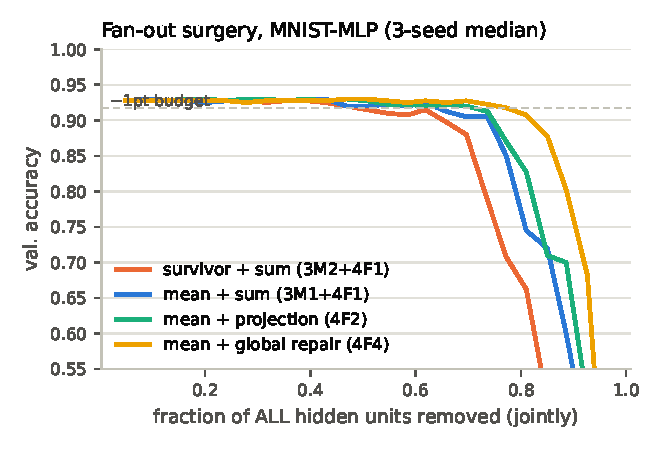
\includegraphics[width=\linewidth]{figs/fig_surgery.pdf}
\end{minipage}\hfill
\begin{minipage}{0.49\textwidth}\centering
  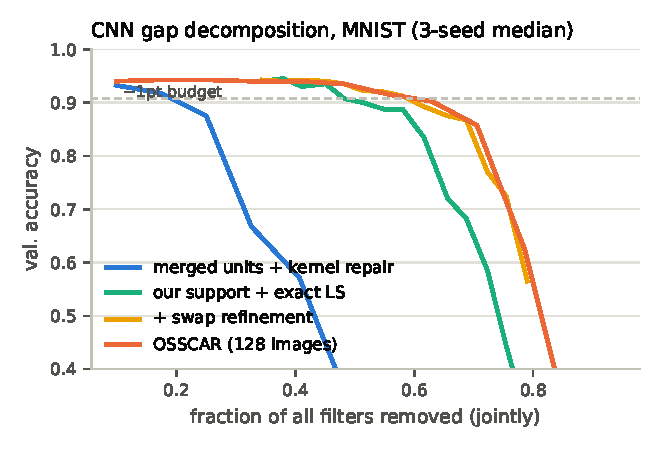
\includegraphics[width=\linewidth]{figs/fig_cnn.pdf}
\end{minipage}
\caption{\textbf{Left (E8):} the fan-out surgery hierarchy on MLPs
(partitions fixed across variants): survivor $<$ mean $<$ projection $<$
global repair (Theorem~\ref{thm:global}), the last worth $+15$ accuracy-
capacity points. \textbf{Right (E10--E13):} the CNN gap decomposition. The
merged-unit/kernel pipeline collapses early; keeping our supports but
switching to the exact-LS repair recovers most of the gap; one swap
refinement pass reaches OSSCAR exactly --- selection was never the problem
(cf.\ the overlap of Table~\ref{tab:cnn}).}
\label{fig:surgery-cnn}
\end{figure}

\begin{table}[t]
\centering\small
\caption{\textbf{E4 (Phase A):} scoring measures on MNIST-MLP layer~0
(medians over 3 seeds). Capacity $=$ fraction of the layer mergeable within
the stated budget. Right: wins--ties--losses vs.\ Ward on layer-local
capacity (5\% budget) over all 30 (dataset, seed, layer) runs.}
\label{tab:phaseA}
\begin{tabular}{@{}lccc c@{}}
\toprule
scoring measure & cap.\ @1\% err & @5\% err & @$-1$pt acc & W--T--L vs Ward \\
\midrule
Ward, sphere (1A1)            & 0.141 & 0.366 & 0.616 & --- \\
Ward, ellipsoid (1A2)         & 0.137 & 0.325 & 0.706 & 6--5--19 \\
expected damage, isotropic (1B1) & 0.031 & 0.063 & 0.146 & 10--1--19 \\
expected damage, box-CLT (1B3)   & 0.031 & 0.055 & 0.146 & 7--0--23 \\
expected damage, matched (1B4)   & \textbf{0.376} & \textbf{0.576} & \textbf{0.769} & \textbf{27--2--1} \\
\bottomrule
\end{tabular}
\end{table}

\begin{table}[t]
\centering\small
\caption{\textbf{E8 (Phase B):} fan-out surgery, joint equal-fraction
pruning of all layers, func\_matched partitions fixed across variants.
Capacity $=$ fraction of \emph{all} hidden units removed within the budget
(3-seed medians). The global repair exceeds even the cross-layer allocation
grid \emph{oracle} under the sum surgery (0.700 on MNIST, E7).}
\label{tab:phaseB}
\begin{tabular}{@{}lcc cc@{}}
\toprule
& \multicolumn{2}{c}{MNIST} & \multicolumn{2}{c}{Fashion} \\
\cmidrule(lr){2-3}\cmidrule(l){4-5}
surgery & @$-0.5$pt & @$-1$pt & @$-0.5$pt & @$-1$pt \\
\midrule
survivor $+$ sum (3M2$+$4F1) & 0.429 & 0.547 & 0.429 & 0.429 \\
mean $+$ sum (3M1$+$4F1)     & 0.585 & 0.618 & 0.469 & 0.547 \\
mean $+$ projection (4F2)    & 0.658 & 0.696 & 0.585 & 0.585 \\
mean $+$ global repair (4F4) & \textbf{0.737} & \textbf{0.772} & \textbf{0.772} & \textbf{0.772} \\
\bottomrule
\end{tabular}
\end{table}

\begin{table}[t]
\centering\small
\caption{\textbf{E9 (Phase D, MLPs):} ours vs.\ OSSCAR at matched data
budgets, joint pruning, capacity within budget (3-seed medians; width grid
resolution $\pm 0.08$). \emph{hybrid128} $=$ our structure with empirical
Grams: identical to the parametric kernel in every cell --- second moments
are sufficient statistics here (Remark~\ref{rem:estimators}).}
\label{tab:phaseD}
\begin{tabular}{@{}lccc ccc@{}}
\toprule
& \multicolumn{3}{c}{MNIST} & \multicolumn{3}{c}{Fashion} \\
\cmidrule(lr){2-4}\cmidrule(l){5-7}
arm & $-0.5$pt & $-1$pt & $-2$pt & $-0.5$pt & $-1$pt & $-2$pt \\
\midrule
ours (128 imgs, moments)  & 0.712 & 0.712 & 0.790 & \textbf{0.790} & 0.790 & 0.790 \\
hybrid128 (empirical)     & 0.712 & 0.712 & 0.790 & 0.790 & 0.790 & 0.790 \\
OSSCAR (128 imgs)         & 0.712 & \textbf{0.790} & 0.790 & 0.712 & 0.790 & 0.790 \\
OSSCAR (full 2000)        & 0.790 & 0.790 & \textbf{0.868} & 0.712 & 0.790 & 0.790 \\
\bottomrule
\end{tabular}
\end{table}

\begin{table}[t]
\centering\small
\caption{\textbf{E10--E13 (Phase D, CNNs):} the gap and its complete
decomposition, capacity @$-1$pt (3-seed medians; fine $\pm0.035$ grid for
the last three rows). Middle: removal-set overlap with OSSCAR at matched
$k$ (E11; chance in parentheses) --- both methods drop largely the same
filters even where capacities diverge, isolating the surgery as the cause.}
\label{tab:cnn}
\begin{tabular}{@{}lcc c@{}}
\toprule
arm & MNIST & Fashion & overlap @25\% (chance 0.25) \\
\midrule
merged units $+$ kernel repair (E10) & 0.174 & 0.326 & 0.50--0.75 \\
our support $+$ exact LS (E12)       & 0.482 & 0.580 & '' \\
$+$ swap refinement (E13)            & \textbf{0.549} & \textbf{0.616} & '' \\
OSSCAR, 128 imgs                     & 0.549 & 0.616 & 1.00 (self) \\
\midrule
MLP reference (E11) & \multicolumn{3}{c}{overlap up to 0.94 at half the
layer removed (chance 0.50)} \\
\bottomrule
\end{tabular}
\end{table}

Figures~\ref{fig:metric-bound}--\ref{fig:surgery-cnn} and
Tables~\ref{tab:phaseA}--\ref{tab:cnn} display the primary results;
raw per-step trajectories live in the repository outputs directory.
Two additional numbers complete the record: on pretrained ResNet-18
(Imagenette, E5), per-block filter counts removable at $-1$pt were
$35/35/71/71/127/143/287/95$ of $64/64/128/128/256/256/512/512$ for Ward and
$47/19/63/47/95/127/255/287$ for the matched measure (task over-provisioning,
not weight-space redundancy: at $5\%$ layer error every arm manages only
$1$--$3\%$ of filters); and stopping-rule transfer (E6) gave
$0.6$--$0.77$ of oracle capacity at zero violations within a domain, with
only the normalized cumulative expected damage transferring safely across
domains ($\approx 0.5$ capture at $0$--$3\%$ violations).

\paragraph{Honest failures and their theoretical meaning.}
Three assumptions failed measurably, each in the direction the theory
anticipates once the assumption is stated: (a) isotropy and independence of
input coordinates (Remark~\ref{rem:measure}) --- falsified wherever inputs
are structured; (b) Gaussianity of conv patch distributions --- falsified,
forcing the empirical estimator on conv models; (c) the existence of cluster
structure in well-trained conv filters --- absent under BatchNorm at scale
(pretrained ResNet-18: $1$--$3\%$ of filters mergeable at $5\%$ layer error),
so that on such models pruning capacity is \emph{task} over-provisioning
rather than weight-space redundancy, and the medoid/subset realization with
data-based repair is the correct operating point. None of these failures
touches the theorems; they locate the boundaries of their hypotheses.

\end{document}
